
\documentclass[12pt, addpoints]{exam}
\usepackage[utf8]{inputenc}
\usepackage[portuguese]{babel}
\usepackage{multicol}
\usepackage{graphicx}
\usepackage{amsmath}
\usepackage{xcolor}
\usepackage[a4paper, portrait, margin=2cm]{geometry}

\setlength{\columnsep}{1cm}

        \begin{document}

\begin{minipage}[l]{0.5\linewidth}
    \begin{flushleft}
        {\bf \Large Prova bimestral}
    \end{flushleft}
\end{minipage}
\begin{minipage}[r]{0.45\linewidth}
    \begin{flushright}
        {\bf \Large Código: XXXXX}
    \end{flushright}
\end{minipage}
\vspace{0.5cm} \hrule \vspace{0.5cm}
\begin{minipage}{0.75\linewidth}
    Aluno:
\end{minipage}
\begin{minipage}{0.20\linewidth}
    Data: 
\end{minipage}
\vspace{0.5cm} \hrule \vspace{0.5cm}

\begin{center}
\textcolor{red}{\emph\Large Correction version}\end{center}
\begin{questions}
\begin{multicols}{2}
\question[33] Durante sua trajetória uma partícula realizou um trabalho de   -3.61 J. Qual foi a variação da sua energia cinética?

\begin{oneparchoices}
\choice -5.94 J\choice -3.61 J\choice -5.15 J\choice -1.34 J\choice -9.88 J\choice 9.0 J\choice 5.94 J\choice -3.52 J\choice -5.76 J\choice -6.65 J\end{oneparchoices}

\begin{oneparchoices}
\choice 0.0\choice 33\choice 0.0\choice 0.0\choice 0.0\choice 0.0\choice 0.0\choice 0.0\choice 0.0\choice 0.0\end{oneparchoices}
\question[23] Considere uma partícula de massa    7.43 kg e velocidade    2.17 m/s. Determine a sua energia cinética.

\begin{center}
\begin{minipage}[c]{0.75\linewidth}
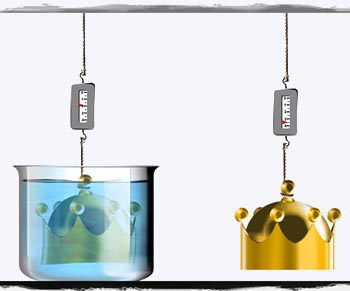
\includegraphics[width=\textwidth]{MWE001.jpg}
\end{minipage}

\end{center}
\begin{oneparchoices}
\choice 40.1 J\choice 536.06 J\choice 68.45 J\choice 218.82 J\choice 721.46 J\choice 19.27 J\choice 13.37 J\choice 115.28 J\choice 360.81 J\choice 17.5 J\end{oneparchoices}

\begin{oneparchoices}
\choice 0.0\choice 0.0\choice 0.0\choice 0.0\choice 0.0\choice 0.0\choice 0.0\choice 0.0\choice 0.0\choice 23\end{oneparchoices}
\end{multicols}
\end{questions}
\newpage
\begin{minipage}[l]{0.5\linewidth}
    \begin{flushleft}
        {\bf \Large Prova bimestral}
    \end{flushleft}
\end{minipage}
\begin{minipage}[r]{0.45\linewidth}
    \begin{flushright}
        {\bf \Large Código: XXXXX}
    \end{flushright}
\end{minipage}
\vspace{0.5cm} \hrule \vspace{0.5cm}
\begin{minipage}{0.75\linewidth}
    Aluno:
\end{minipage}
\begin{minipage}{0.20\linewidth}
    Data: 
\end{minipage}
\vspace{0.5cm} \hrule \vspace{0.5cm}

\begin{center}
\textcolor{red}{\emph\Large Correction version}\end{center}
\begin{questions}
\begin{multicols}{2}
\question[33] Durante sua trajetória uma partícula realizou um trabalho de    8.14 J. Qual foi a variação da sua energia cinética?

\begin{oneparchoices}
\choice -5.11 J\choice 9.05 J\choice 1.83 J\choice 5.57 J\choice -8.1 J\choice 6.87 J\choice -0.08 J\choice 3.08 J\choice 8.14 J\choice -3.41 J\end{oneparchoices}

\begin{oneparchoices}
\choice 0.0\choice 0.0\choice 0.0\choice 0.0\choice 0.0\choice 0.0\choice 0.0\choice 0.0\choice 33\choice 0.0\end{oneparchoices}
\question[23] Considere uma partícula de massa    8.91 kg e velocidade    3.36 m/s. Determine a sua energia cinética.

\begin{center}
\begin{minipage}[c]{0.75\linewidth}
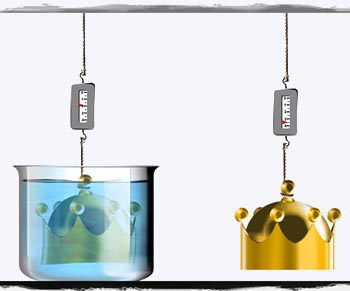
\includegraphics[width=\textwidth]{MWE001.jpg}
\end{minipage}

\end{center}
\begin{oneparchoices}
\choice 2.67 J\choice 251.55 J\choice 286.24 J\choice 140.43 J\choice 146.87 J\choice 50.36 J\choice 159.92 J\choice 257.97 J\choice 100.2 J\choice 279.96 J\end{oneparchoices}

\begin{oneparchoices}
\choice 0.0\choice 0.0\choice 0.0\choice 0.0\choice 0.0\choice 23\choice 0.0\choice 0.0\choice 0.0\choice 0.0\end{oneparchoices}
\end{multicols}
\end{questions}
\newpage\end{document}